% !TeX root = RJwrapper.tex
\title{SIQR: An R Package for Single-index Quantile Regression}
\author{by Tianhai Zu and Yan Yu}

\newcommand{\fixup}[1]{\marginpar{\flushleft{#1}}}
\newcommand{\ut}{\underline{t}}
\newcommand{\uYi}{\underline{Y}_i(\underline{t})}
\newcommand{\udi}{\underline{\delta}_i}
\newcommand{\umi}{\underline{\mu}_i}
\renewcommand{\theequation}{\arabic{equation}}

%%%%%%%%%%%%%%%%%%%new added definition


\def\bef{{\bf f}}
\def\bzero{{\bf 0}}
\def\bA{{\bf A}}
\def\bB{{\bf B}}
\def\bBz{{\bB}_z}
\def\bBzt{{\bB}^T_z}
\def\bx{{\bf x}}
\def\bX{{\bf X}}
\def\by{{\bf y}}
\def\bY{{\bf Y}}
\def\bz{{\bf z}}
\def\bZ{{\bf Z}}
\def\bv{{\bf v}}
\def\bG{{\bf G}}
\def\bC{{\bf C}}
\def\bD{{\bf D}}
\def\bI{{\bf I}}
\def\bG{{\bf G}}
\def\bL{{\bf L}}
\def\bS{{\bf S}}
\def\bW{{\bf W}}
\def\be{{\bf e}}
\def\bN{{\bf N}}
\def\b0{\bmath{0}}
\def\bM{{\bf M}}
\def\bO{{\bf O}}
\def\bP{{\bf P}}
\def\bQ{{\bf Q}}
\def\bu{{\bf u}}
\def\bT{{\bf T}}
\def\bU{{\bf U}}
\def\bJ{{\bf J}}
\def\bv{{\bf v}}
\def\bV{{\bf V}}
\def\bH{{\bf H}}
\def\bR{{\bf R}}
\def\bOmega{\bmath{\Omega}}
\def\blambda{\bmath{\lambda}}
\def\btheta{\bmath{\theta}}
\def\bphi{\bmath{\phi}}
\def\bphihat{\widehat{\bphi}}
\def\bthetahat{\widehat{\btheta}}
\def\bmath#1{\mbox{\boldmath$#1$}}
\def\transpose{{\sf T}}
\def\trans{^{\transpose}}
\def\inv{^{-1}}
\def\balpha{\bmath{\alpha}}
\def\bgamma{\bmath{\gamma}}
\def\balphahat{\widehat{\balpha}}
\def\bPalpha{{\bf P_{\balphazero}}}
\def\bPalphahat{{\bf P_{\balphahat}}}
\def\bbeta{\bmath{\beta}}
\def\bbetahat{\widehat{\bbeta}}
\def\eps{\epsilon}
\def\bpsi{\bmath{\psi}}
\def\bz{{\bf z}}
\def\bdelta{\bmath{\delta}}
\def\bdeltahat{\widehat{\bdelta}}

\maketitle

\abstract{We develop an R package \pkg{SIQR} that implements the single-index quantile regression (SIQR) models via an efficient iterative local linear approach in \cite{wu_single-index_2010}. Single-index quantile regression models are important tools in semiparametric regression to provide a comprehensive view of the conditional distributions of a response variable. It is especially useful when the data is heterogeneous or heavy tailed. The package provides functions that allow users to fit SIQR models, predict, provide standard errors of the single-index coefficients via bootstrap, and visualize the estimated univariate function. We apply the R package \pkg{SIQR} to a well-known Boston Housing data.
}

\section{Introduction}

Single-index quantile regression \citep{wu_single-index_2010} generalizes the seminal work of linear quantile regression of \cite{koenker_regression_1978} by projecting the $d$-dimensional covariate $\bx$ to a univariate index $\bx\bbeta$ and allowing a flexible univariate function $g(\bx\bbeta).$ Quantile regression is often of great interest, especially when heterogeneity is present. Applications lie in a variety of fields, such as growth curves and reference
charts in medicine; survival analysis when a given covariate may have a different effect on individuals with different level of risks; value at risk calculation and wage and income studies in financial economics; high peak electricity demand in terms of weather characteristics in utility and energy; modeling rainfall, river flow, and air pollution in environmental modeling (see a survey in\citealt{yu_quantile_2003}). 

Single-index quantile regression (SIQR) is a flexible semiparametric quantile regression model for analyzing heterogeneous data. The SIQR model has some appealing features: (i)
By examining the full spectrum of conditional quantiles, it can provide a comprehensive view of the conditional distribution of a response variable given $d$-dimensional covariates. This is especially important for complex heterogeneous data. (ii) The single-index structure is flexible to accommodate nonlinearity while avoiding the curse of dimensionality. It can also implicitly model some interactions among the covariates. Some interesting interpretation of the single-index parameter may be preserved. (iii) The quantile regression approach is robust to heavy-tailed distributions.

We present a package \pkg{SIQR} in R that implements the iterative local linear approach to the single-index quantile regression in \cite{wu_single-index_2010}. The unknown univariate function is estimated by local linear estimation. The key algorithm can be decomposed into two efficient estimation steps on augmented data through local linear approximation and some equivalent formulation of the expected loss. Essentially, it iterates between two linear quantile regressions utilizing the state-of-the-art R package \pkg{quantreg}. 

We apply our R package \pkg{SIQR} to the well-known Boston Housing data (1978) that is available in R default library. The data has a total of 506 observations and the response variable of interest is the median price of owner-occupied homes on the census
tracts in suburban Boston from the 1970 census.
The response variable and some covariates are left-skewed. Clearly, quantile regression is a natural tool to analyze the data (e.g., \citealt{chaudhuri_average_1997}; \citealt{yu_local_2004}; \citealt{wu_single-index_2010}; \citealt{kong_single-index_2012}). We organize the rest of the paper as follows. In the next section, we review the SIQR models. Next, we discuss the estimation algorithms implemented in this package.  The section following describes the main features of the functions provided. Section ``Real Data Analysis and Simulation'' illustrates the use of \textbf{SIQR} in R for Boston housing data and a simulation study. The last section concludes the paper.

\section{An overview for single-index quantile regression}


\subsection{Data structure and model settings}

We develop an R package for the single-index quantile regression for semiparametric estimation with $d$-dimensional covariates.
Let $Y$ be the response variable and $\bX$ be the covariate vector. 
Suppose there are $n$ observations $\bigl\{(\bx_i,y_i)\bigr\}_{i=1}^n$ of $(\bX=\bx,Y=y)$. Given $\tau\in(0,1)$ and covariates $\bx_i$, the single-index quantile model for the $\tau$-th conditional quantile of the $i$-th observation is
\begin{equation} \label{eq:siqr}
q_{\tau}(Y=y_i | \bX=\bx_i) = g_\tau (\bx_i \bbeta_{\tau}),
\end{equation}
where $y_i$ is a real valued response; covariate $\bx_i$ is a $d$-dimensional row vector; the single-index parameter $\bbeta_{\tau}$ is a column vector in ${\bf R}^d$, and the univariate function $g_{\tau}: \bR \rightarrow \bR$ is subject to different $\tau$.
	For identifiability, the single index parameter $\|\bbeta_{\tau}\|= 1$ and the first non-zero element of $\bbeta_{\tau}$ is positive \citep{yu_penalized_2002}. The projection $\bx\bbeta$ is often termed as the "single index".
When $g_{\tau}$ is linear, single-index quantile regression model (\ref{eq:siqr}) reduces to the seminal work of linear quantile regression of \cite{koenker_regression_1978}.


\subsection{Review of local linear estimation for single-index quantile regression} \label{sec:single-index model}

We implement the local linear estimation for single-index quantile regression (\ref{eq:siqr}) \citep{wu_single-index_2010}. For notational convenience, we omit the subscript $\tau$ in $g_\tau$ and $\bbeta_{\tau}$. The true parameter vector $\bbeta$ is the minimizer of
%eq loss 1
\begin{equation}\label{eq loss1}
 E\left[\rho_\tau\left(y-g(\bx\bbeta)\right)\right] ,
\end{equation}
where $\rho_\tau(u)=|u|+(2\tau-1)u$ is
the loss function, often termed as the ``check" function in quantile regression. $g(\cdot)$ is the unknown univariate function. And constraint $\|\bbeta\|=1, \beta_1>0$ is imposed for identifiability. The above expected loss can be equivalently written as
\begin{equation}\label{eq loss2}
E\left\{E\left[\rho_\tau\left(y-g(\bx\bbeta)\right)|\bx\bbeta\right]\right\}, \end{equation}  where $E\left[\rho_\tau\left(y-g(\bx\bbeta)\right)|\bx\bbeta\right]$ is the conditional expected loss and $g(\cdot)$ is the $\tau$th conditional quantile given the single-index parameter $\bbeta$.

We adopt a local linear approximation. In particular, for $\bx_i\bbeta$ "close'' to $u$, we can approximate the $\tau$th conditional quantile at $\bx_i\bbeta$ linearly via
\begin{equation*} 
%\label{eq:g approx}
g(\bx_i\bbeta)\approx g(u)+g'(u)(\bx_i\bbeta-u)=a+b(\bx_i\bbeta-u),
\end{equation*}
where we define $a{\equiv}g(u)$ and $b{\equiv}g'(u)$.

Now we can minimize the sample analogue of (\ref{eq loss1}) below as in \cite{yu_local_1998} with respect to $(a, b)$ with local linear estimation
\begin{equation}\label{eq condloss}\sum_{i=1}^n\rho_\tau\left(y_i-a-b(\bx_i\bbeta-u)\right)K\left(\frac{\bx_i\bbeta-u}{h}\right),
\end{equation}
where $K(\cdot)$ is the kernel function and $h$ is the bandwidth.

We further average (\ref{eq condloss}) over $u$ and obtain the sample analog of (\ref{eq loss2}). The objective function below is used to estimate our single-index quantile regression model~(\ref{eq:siqr}),
\begin{equation} \label{eq total loss}
%& & \sum_{j=1}^nv_j\sum_{i=1}^n\rho_\alpha\left(y_i-a_j-b_j(X_i-X_j)^T\gamma\right)\omega_{ij}\\
\sum_{j=1}^n\sum_{i=1}^n\rho_\tau\left(y_i-a_j-b_j(\bx_i\bbeta-\bx_j\bbeta)\right)\omega_{ij},
\end{equation}
where 
\begin{equation} \label{eq wij} \omega_{ij}=\frac{K_h(\bx_i\bbeta-\bx_j\bbeta)}{\sum_{k=1}^n K_h(\bx_k\bbeta-\bx_j\bbeta)}
\end{equation}
and $K_h(\cdot)=K(\cdot/h)/h.$
We implement minimizing (\ref{eq total loss}) iteratively with detailed algorithm described next.

Bandwidth is a critical smoothing parameter that tunes the smoothness of the fitted function in local estimation. We implement the choice of the optimal bandwidth  $h_\tau$ as advocated in \cite{wu_single-index_2010} through a computationally-expedient rule-of-thumb:
\begin{equation}\label{eq approx hp}
h_{\tau}=h_m\left\{\tau(1-\tau)/\phi\left(\Phi^{-1}(\tau)\right)^2\right\}^{1/5},
\end{equation}
where $\phi(\cdot)$ is the probability density function and $\Phi(\cdot)$ is the cumulative distribution function of the standard normal distribution. Here $h_m= \Bigl\{ \frac{[ \int K^2(v)dv ] [var(y|\bx\bbeta=u)]}{n [ \int v^2 K(v)dv ]^2 [\frac{d^2}{d u^2}E(y|\bx\bbeta=u)]^2 [f_{U_0}(u)]} \Bigr\}^{1/5}$ is the optimal bandwidth in mean regression, which is easily obtainable from many existing packages \citep{ruppert_effective_1995}. 
%$f_{U_0}(\cdot)$ is the density of $U_0$.

\subsection{Algorithm}

We present the main algorithm for fitting the single-index quantile regression (SIQR) with local linear estimation in detail as following: 

\begin{algorithm}[H]  
	\KwIn{Quantile level $\tau\in(0,1)$, $d$-dimensional covariate vector $\bX=\mathbf{x}$, and a response vector $Y=\mathbf{y}$.}
	\KwOut{The estimated quantile single-index parameter $\widehat{{\bbeta}}_{\tau}$ and fitted conditional quantile $\hat{q}_{\tau}(Y =\by | \bX=\bx)$. The univariate function estimate $\hat{g}_{\tau}(\cdot)$}
	
	Obtain an initial estimate $\hat{\bbeta}^{(0)}$ of the quantile single-index parameter $\bbeta$ from a linear quantile regression model (default), or a user-provided initial list.
	Standardize the initial estimate such that $||{\hat {\bbeta}}^{(0)}||=1$ and ${\hat {\beta}}^{(0)}_1>0.$ 
	
	Given $\hat {\bbeta}$, obtain $\{{\hat a}_j, {\hat b}_j\}_{j=1}^n$ by solving a series of the following
		\begin{equation}\label{eq:step2}
		\min_{(a_j, b_j)}\sum_{i=1}^n\rho_\tau\left(y_i-a_j-b_j(\bx_i-\bx_j){\hat{\bbeta}}\right)\omega_{ij},
		\end{equation}
		where the weights $\omega_{ij}$ is defined in (\ref{eq wij}). The bandwidth $h$ is chosen optimally following a rule-of-the-thumb criterion in (\ref{eq approx hp}).
		
	Given  $\{{\hat a}_j, {\hat b}_j \}_{j=1}^n$, obtain ${\hat{\bbeta}}$ by solving
		\begin{equation} 
		\min_{\bbeta}\sum_{j=1}^n\sum_{i=1}^n\rho_\tau\left(y_i-{\hat a}_j-{\hat b}_j (\bx_i-\bx_j)\bbeta\right)\omega_{ij}, \label{eq:step3}
		\end{equation}
		with $\omega_{ij}$ evaluated at ${\bbeta}$ and $h$ from step 2.
		
	    Repeat Steps 2 and 3 until convergence.
	    
	    Finally, we estimate $g(\cdot)$ at any $u$ by $\hat{g}(\cdot;h, \hat{\bbeta})=\hat{a}$ where
	    \begin{equation*}\label{eq final link}
	    (\hat{a},\hat{b})=\arg\min_{(a, b)}\,\sum_{i=1}^n\rho_\tau\left(y_i-a-b(\bx_i{\hat{\bbeta}}-u)\right)K_h(\bx_i\hat{\bbeta}-u).
	    \end{equation*}
	    Obtain the final fitted conditional quantile $\hat{q}_{\tau}(Y =\by | \bX=\bx)$ from model~(\ref{eq:siqr}).
	
\end{algorithm}


The above algorithm effectively decomposes (\ref{eq total loss}) into two steps that can be achieved by two standard linear quantile regression procedures in  Steps 2 and 3. In Step 3, we further note that (\ref{eq:step3}) can be written as
\begin{eqnarray*}
	\hat{\bbeta}&=&\arg\min_{\bbeta} \sum_{j=1}^n\sum_{i=1}^n\rho_\tau\left(y_i-{\hat a}_j-{\hat b}_j(\bx_i-\bx_j)\bbeta\right)\omega_{ij}
	\\&=&\arg\min_{\bbeta}\sum_{j=1}^n\sum_{i=1}^n\rho_\tau\left(y_{ij}^*-{\bx_{ij}^*}\bbeta\right)\,\omega_{ij},
\end{eqnarray*}
where $y_{ij}^*=y_i-{\hat a}_j$, $\bx_{ij}^*={\hat a}_j(\bx_i-\bx_j)$, and $\omega_{ij}$ evaluated at the previous step, $i,j=1,\cdots,n$.
Given ${\hat a}_j$'s and ${\hat b}_j$'s, we can estimate $\bbeta$ through usual linear quantile regression without intercept ({\it regression-through-origin}) on $n^2$ "observations" $\{y_{ij}^*,{\bx}_{ij}^*\}_{i,j=1}^n$ with known weights $\{\omega_{ij}\}_{i,j=1}^n$ evaluated at the estimate of $\bbeta$ from the previous iteration.

We can see that (\ref{eq:step3}) is an alternative of (\ref{eq:step2}). Adopting (\ref{eq:step3}) yields some  advantages: (i) It uses all the data and is more efficient in estimation; (ii) The double sum in (\ref{eq:step3}) effectively increases the "augmented" sample size to $n^2$ similar as the minimum average variance
estimation (MAVE) in the mean regression \citep{xia_semi-parametric_2006}.


\section{The SIQR package}
The R package SIQR consists of one core estimation function \textbf{siqr} and some supporting functions such as visualization tool \textbf{plot.siqr} and summary function \textbf{summary.siqr}. The R package SIQR depends on the R packages \pkg{stats}, \CRANpkg{quantreg}, \CRANpkg{KernSmooth}.

\subsection{Main fitting function}

The main estimation function \textbf{siqr} implements the iterative local linear approach to the single-index quantile regression in \cite{wu_single-index_2010}. 

The usage and input arguments of the main fitting function \textbf{siqr} are summarized as follows:

\begin{example}
  siqr(y, X, tau=0.5, gamma.inital=NULL, se.method = NULL, maxiter=50, tol=1e-8)
\end{example}

This function takes two required arguments: the response variable Y in vector format, the covariate matrix X. Please note that all the input covariates are required to be numeric variables. 

This function also takes several optional arguments for finer controls. The optional argument \textbf{tau} is the quantile index, which specifies the left-tail probability. The default value of \textbf{tau} is 0.5, which refers to a single-index median regression.  The optional argument \textbf{user.init} is a numeric vector of the same length as the dimensionality of covariates. The users can use this argument to pass in any appropriate user-defined initial single-index coefficients based on prior information or domain knowledge. The default value is NULL, which instructs the function to estimate the initial single index coefficients by linear quantile regression. The optional argument \textbf{se.method} is a character variable that specifies the method to obtain standard error of estimated single-index coefficients. The default value is NULL to skip the calculation of standard error while bootstrap based method is available with "bootstrap". The optional argument \textbf{maxiter} and \textbf{tol} control parameter that specifies the criteria to terminate the iteration process. Although the algorithm normally converges quickly, the default \textbf{maxiter} and \textbf{tol} are set to 50 and 1e-8, respectively.

\subsection{Other functions}

We also provide several supporting functions:

\begin{example}
  summary.siqr(siqr.object)
  print.summary.siqr(siqr.object)
\end{example}
The functions \textbf{summary.siqr} and \textbf{print.summary.siqr} provide detailed information related to the fiited model and summarize the results as illustrated in the next section. These two functions can be called directly by applying functions print and summary to the siqr.object. 

\begin{example}
  plot.siqr(siqr.object, data.points = TRUE, bootstrap.interval=FALSE)
\end{example}
This function plots the fitted quantiles against the single-index term from a siqr-fitted model object. By default, this function will also plot the observed data points in addition to the fitted quantiles to visualize the fitness of the model. One can remove the data points by setting the optional argument \textbf{data.points} to FALSE. Point-wise confidence interval will be added to the plot if the optional arugument \textbf{bootstrap.interval} is set to TRUE. 



\begin{example}
  simulation_data <- generate.data(n, true.theta=NULL, sigma=0.1, 
  setting="setting1", ncopy=1)
\end{example}

To help perform simulation studies, the function \textbf{generate.data} generates a size $n$ data from two different settings: (i) a sine-bump model; and (ii) a location-scale model as in \cite{wu_single-index_2010}. Users can define the single-index coefficients $\boldsymbol{\theta}$ via the argument \textbf{true.beta} and the noise level via \textbf{sigma}. If no \textbf{true.beta} was provided, the function will use $(1,1,1)^{\intercal} / \sqrt{3}$ for setting 1 and $(1,2)^{\intercal} / \sqrt{5}$ for setting 2 as the default. The last optional argument \textbf{ncopy} generates multiple copies of data for Monte Carlo simulations. 

\section{Real Rata and Simulations}

\subsubsection{Boston Housing data}

We consider the Boston housing data to demonstrate the real data application of the proposed R package \pkg{SIQR}. This dataset contains the median value of houses (in \$1000's), medv, in 506 tracts in Boston and 13 other socio-demographic related variables. This data has been investigated by many studies. Heterogeneity and some non-linear dependence of medv on predictor variables has been found by previous researchers. The dataset is maintained at the StatLib library of Carnegie Mellon University and can be found at the R built-in package \pkg{MASS}.

We focus on the following four covariates: RM, average number of rooms per dwelling; TAX, full-value property tax (in \$) per \$10,000; PTRATIO, pupil-teacher ratio by town; and LSTAT, percentage of lower status of the population as in \cite{opsomer_fully_1998}, \cite{yu_local_2004} and \cite{wu_single-index_2010}. Following previous studies, we take logarithmic transformations on TAX and LSTAT and center the dependent variable medv around zero.

We use the following codes to load data from \pkg{MASS} and pre-process as discussed above. We fit a single-index quantile regression with $\tau = 0.25,0.50,0.75$ to the data and report fitted single-index coefficients for each variable.
\begin{Schunk}
  \begin{Sinput}
  library(SIQR)
  #load data from MASS
  library(MASS)
  medv<- Boston$medv
  RM <- Boston$rm
  logTAX <- log(Boston$tax)
  PTRATIO <- Boston$ptratio
  logLSTAT <- log(Boston$lstat)

  X <- cbind(RM,logTAX,PTRATIO,logLSTAT)
  y0 <- medv - mean(medv)
  beta0 <- NULL
  tau.vec <- c(0.25,0.50,0.75)
  est.coefficient <- matrix(NA, nrow = length(tau.vec), ncol = 5)
  est.coefficient[,1] <- tau.vec
  for (i in 1:length(tau.vec)){
  est <- siqr(y0,X,beta.inital = beta0, tau=tau.vec[i],maxiter = 20,tol = 1e-6)
  est.coefficient[i,2:5] <- est$beta
  }
  colnames(est.coefficient) <- c("quantile tau",colnames(X))
  est.coefficient
\end{Sinput}
\begin{Soutput}
 #>      quantile tau        RM     logTAX     PTRATIO   logLSTAT
 #> [1,]         0.25 0.3354766 -0.5243753 -0.06850000 -0.7796113
 #> [2,]         0.50 0.3041920 -0.4281384 -0.06305787 -0.8486392
 #> [3,]         0.75 0.1962127 -0.1953405 -0.08930334 -0.9567484
\end{Soutput}
\end{Schunk}

The estimated 0.25, 0.50 and 0.75 quantiles and their 95\% point-wise confidence bounds are plotted with the following codes and outputs.  

\begin{Schunk}
\begin{Sinput}
  est.tau25 <- siqr(y0,X,beta.inital = NULL, tau=0.25)
  plot.siqr(est.tau25,bootstrap.interval = TRUE)
\end{Sinput}

\centering
\addtolength{\leftskip} {-2cm}
\addtolength{\rightskip}{-2cm}
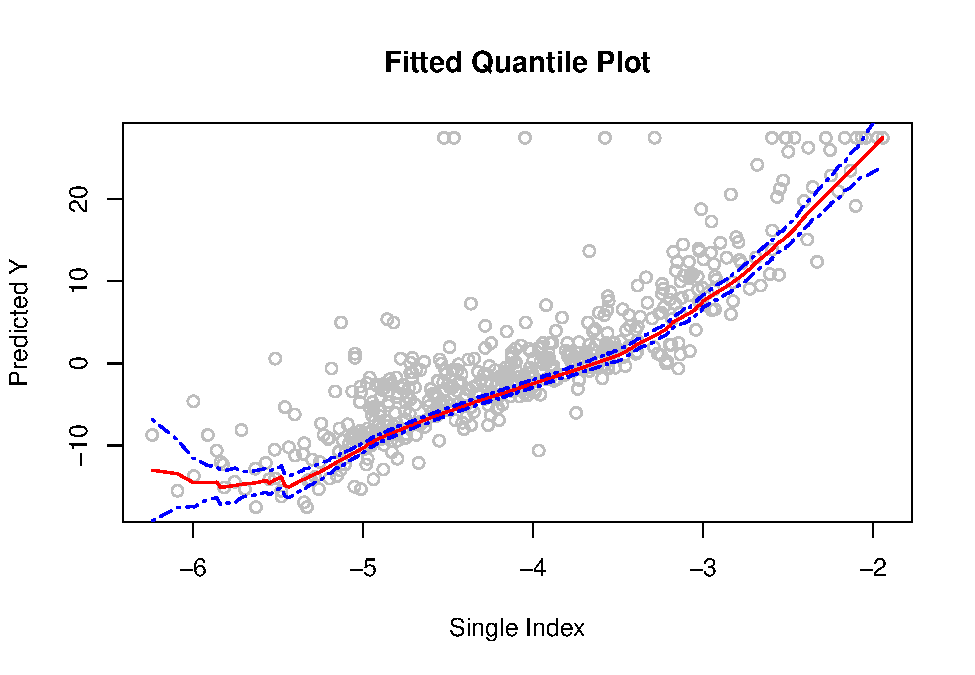
\includegraphics[width=10cm]{siqr_files/figure-latex/unnamed-chunk-2-1} 


\begin{Sinput}
  est.tau50 <- siqr(y0,X,beta.inital = NULL, tau=0.50)
  plot.siqr(est.tau05,bootstrap.interval = TRUE)
\end{Sinput}

\centering
\addtolength{\leftskip} {-2cm}
\addtolength{\rightskip}{-2cm}
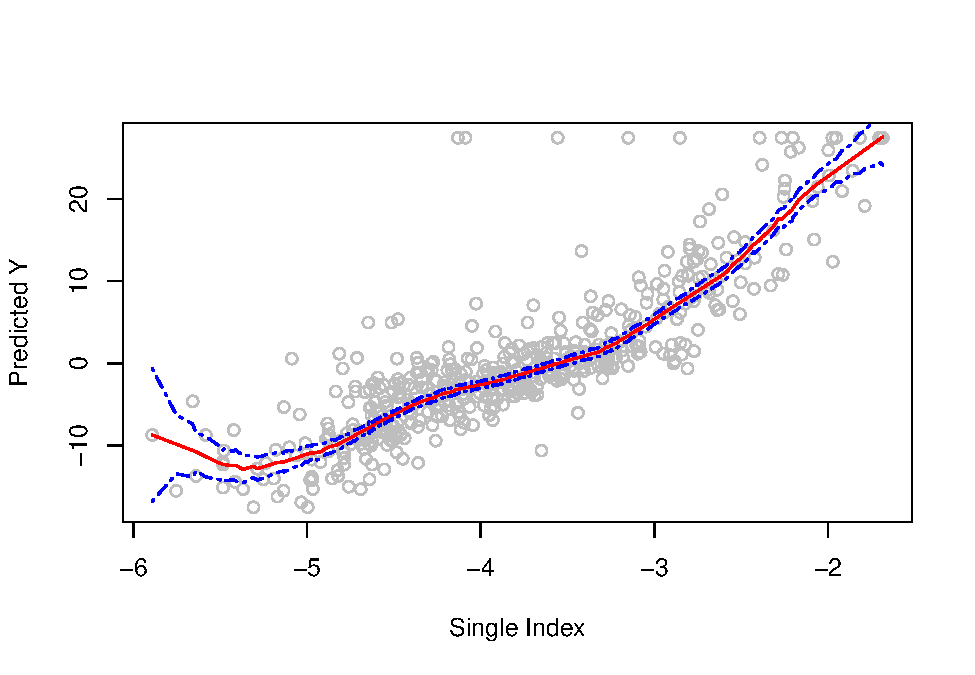
\includegraphics[width=10cm]{siqr_files/figure-latex/unnamed-chunk-3-1} 

\begin{Sinput}
  est.tau75 <- siqr(y0,X,beta.inital = NULL, tau=0.75)
  plot.siqr(est.tau75,bootstrap.interval = TRUE)
\end{Sinput}

\centering
\addtolength{\leftskip} {-2cm}
\addtolength{\rightskip}{-2cm}
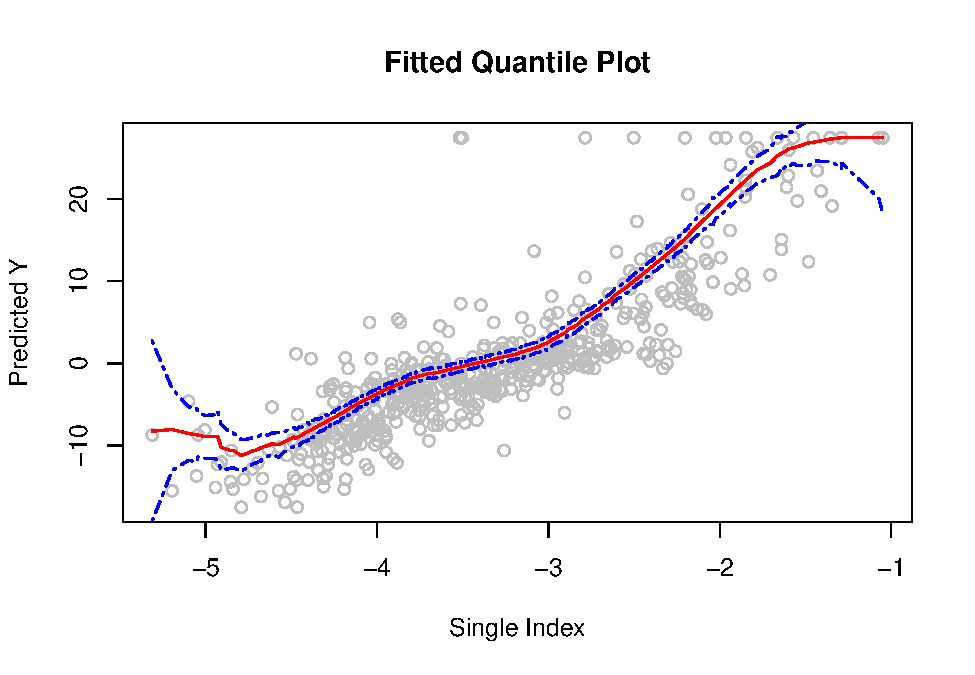
\includegraphics[width=10cm]{siqr_files/figure-latex/unnamed-chunk-4-1} 

\end{Schunk}

As the estimated single-index function curves are almost monotonically increasing across different quantiles, variables that contribute positively to the single-index affect the response variable (medv) positively. Based on the estimated coefficients and above plots, we found that the number of rooms per house (rm) positively affects different quantiles. This matches the intuition that people value large spaces and multi-functional rooms. The property tax rate ln(tax) has a negative impact on housing prices across different quantiles. However, the influence of the tax rate is not significant at higher quantile $\tau$ = 0.75. That suggests tax rate may be less concerned for higher-income households, possibly due to tax deduction towards their income tax. Both the pupil-teacher ratio (ptratio) and the percentage of lower (educational) status of the population ln(lstat) show negative influences on housing values, especially for the higher quantiles. Potential buyers seek areas associated with low risk related to adults without higher education degrees and a better educational environment for their children. 

\subsubsection{Simulation}

We consider two simulation settings. In the first simulation example, we use a sine-bump model with homoscedastic errors:
\begin{equation} \label{eq:sim1}
	y=5 \sin \left(\frac{\pi \left( \bx\bbeta - A \right)}{C-A} \right)+ 0.1 Z, 
\end{equation}
where $A=\frac{\sqrt{3}}{2}-\frac{1.645}{\sqrt{12}}, C=\frac{\sqrt{3}}{2}+\frac{1.645}{\sqrt{12}}$,  $\bx$ is an $n\times3$ design matrix that draws from an independent uniform distribution with min of 0 and max of 1, and the residual $Z$ follows a standard normal distribution. The true single-index parameter $\bbeta = (1,1,1)^{\intercal} / \sqrt{3}$.


\begin{table}[!ht]
	\caption{Summary of parameter estimates for sine-bump simulation example 1 of sample size $n=400$. True  $\bbeta = (1,1,1)^{\intercal} / \sqrt{3}$. The sample mean, standard error (s.e., in parenthesis), and bias of the parameter estimates of single index coefficients from 200 replications.}
	\centering
	\addtolength{\leftskip} {-2cm}
	\addtolength{\rightskip}{-2cm}
	
	\begin{tabular}{llrrr}
		\hline
		& Estimate & $\hat{\beta}_1$ & $\hat{\beta}_2$ & $\hat{\beta}_3$ \\ \hline
		& mean     & 0.5782          & 0.5727          & 0.5725          \\
		$\tau = 0.25$ & s.e.     & 0.0131          & 0.0281          & 0.0293          \\
		& bias     & 0.0009          & -0.0046         & -0.0048         \\
		& mean     & 0.5787          & 0.5755          & 0.5774          \\
		$\tau = 0.50$ & s.e.     & 0.0115          & 0.0105          & 0.0111          \\
		& bias     & 0.0014          & -0.0018         & 0.0003          \\
		& mean     & 0.5803          & 0.5756          & 0.5757          \\
		$\tau = 0.75$ & s.e.     & 0.0119          & 0.0110          & 0.0118          \\
		& bias     & 0.0029          & -0.0017         & -0.0016         \\ \hline
	\end{tabular}
	
	\label{tb:sim1}	
\end{table}

The single index coefficients are estimated via a series of quantile regressions with $\tau = 0.25, 0.50, 0.75$ presented. Table~\ref{tb:sim1} reports the mean, standard error (se), and bias for each parameter estimate with sample size $n=400$ over $M=200$ replications on the simulation example 1.  One can see that the algorithm for our R package \pkg{SIQR} is effective as the estimates are close to the true values. 

For demonstration purpose, we show codes to generate data from (\ref{eq:sim1}) and fit SIQR model using $\tau = 0.50$ with 200 replications as following:

\begin{Schunk}
\begin{Sinput}
 n <- 400
 beta0 <- c(1, 1, 1)/sqrt(3)
 n.sim <- 200
 tau <- 0.50
 data <- generate.data(n, true.theta=beta0, setting = "setting1",ncopy = n.sim)
 sim.results.50 <- foreach(m = 1:n.sim,.combine = "rbind") %do% {
 X <- data$X
 Y <- data$Y[[m]]
 est <- siqr(Y, X, beta.inital = c(2,1,0), tau=0.50,maxiter = 30,tol = 1e-8)
 return(est$beta)
}
\end{Sinput}
\end{Schunk}

Note that this process has been repeated for the cases with $\tau = 0.25, 0.75$. We obtain a box plot of estimated single-index coefficients for $\tau = 0.25, 0.50, 0.75$ respectively by applying the following code snippet. 

\begin{Schunk}
\begin{Sinput}
 boxplot(data.frame((sim.results.25)), outline=T,notch=T,range=1,
 main = "Boxplots of Coefficient Estimates, tau = 0.25",horizontal = F)
\end{Sinput}


\centering
\addtolength{\leftskip} {-2cm}
\addtolength{\rightskip}{-2cm}
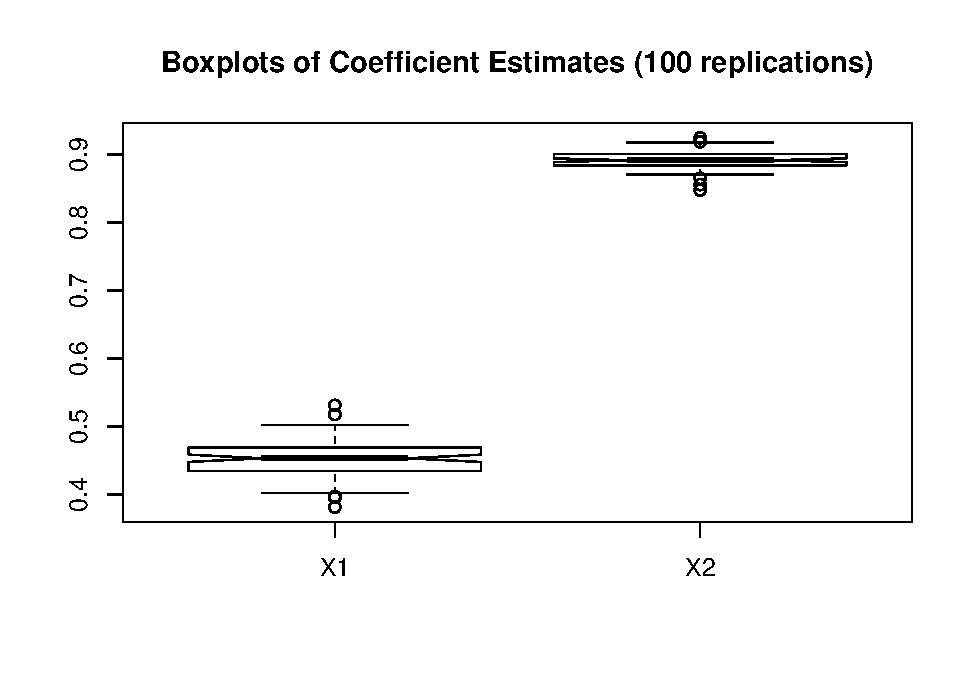
\includegraphics[width=10cm]{siqr_files/figure-latex/unnamed-chunk-7-1}

\begin{Sinput}
 boxplot(data.frame((sim.results.50)), outline=T,notch=T,range=1,
 main = "Boxplots of Coefficient , tau = 0.50",horizontal = F)
\end{Sinput}


\centering
\addtolength{\leftskip} {-2cm}
\addtolength{\rightskip}{-2cm}
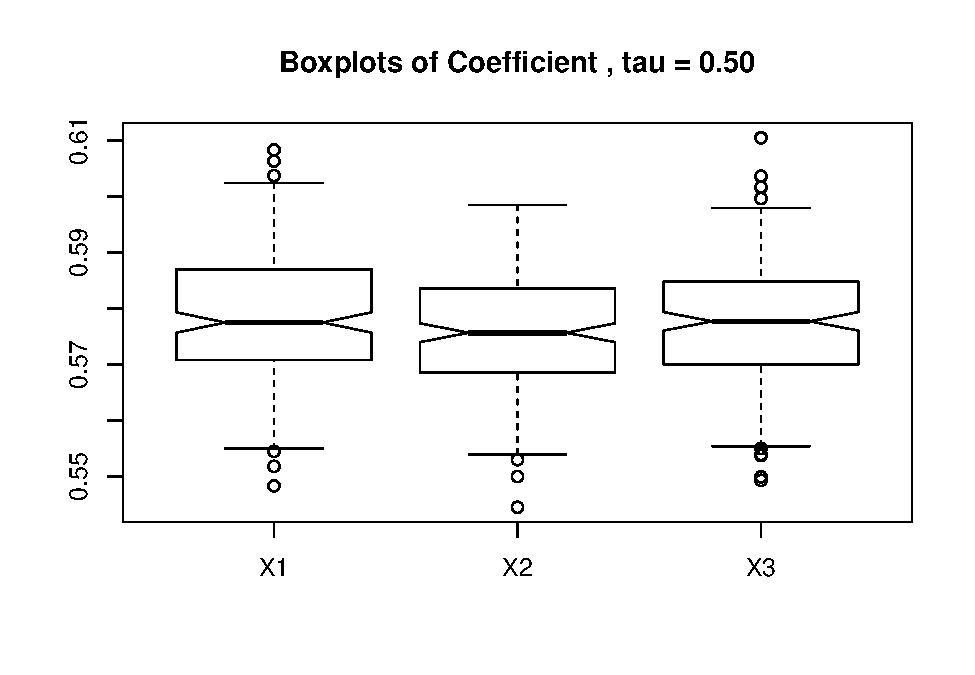
\includegraphics[width=10cm]{siqr_files/figure-latex/unnamed-chunk-8-1}

\begin{Sinput}
 boxplot(data.frame((sim.results.75)), outline=T,notch=T,range=1,
 main = "Boxplots of Coefficient Estimates, tau = 0.75",horizontal = F)
\end{Sinput}

\centering
\addtolength{\leftskip} {-2cm}
\addtolength{\rightskip}{-2cm}
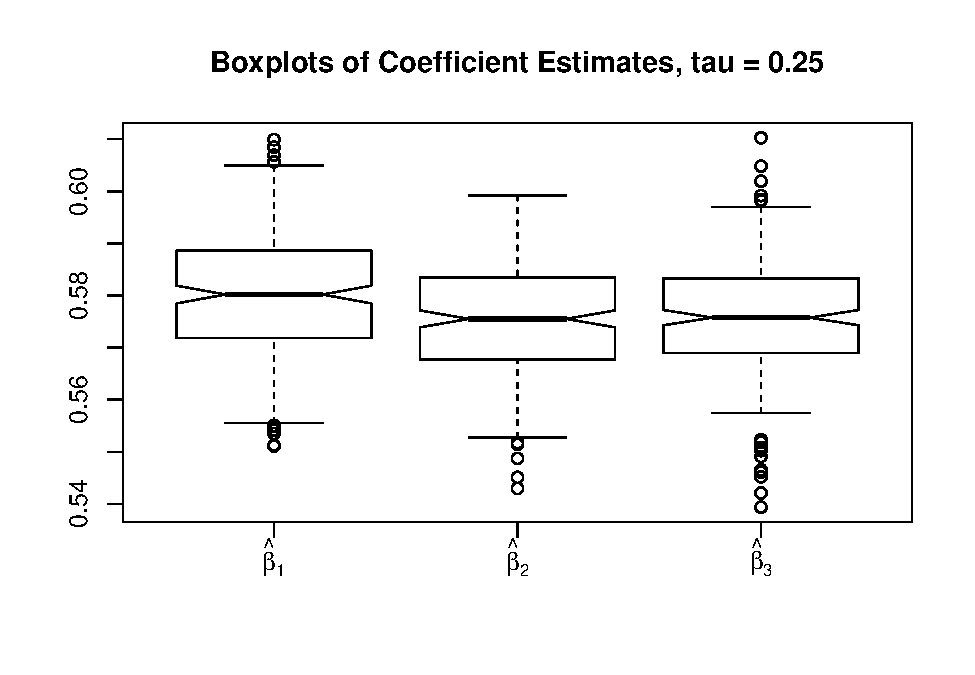
\includegraphics[width=10cm]{siqr_files/figure-latex/unnamed-chunk-9-1} 

\end{Schunk}

\addtolength{\leftskip} {0cm}
\addtolength{\rightskip}{0cm}

Next, we consider a location-scale model as simulation example 2, where both the location and the scale depend on a common index u. The quantiles are ``almost-linear-in-index'' as in \cite{yu_local_1998} when the single index u is close to zero:
\begin{equation} \label{eq:sim2}
  y=5 \cos (\bx\bbeta)+ \exp(-(\bx\bbeta)^2) + E, 
\end{equation}
where $\bx$ is a $n\times2$ design matrix that draws from an independent normal distribution with standard deviation of 0.25 and the residual $E$ follows an exponential distribution with mean 2. The single-index parameter $\bbeta = (1,2)^{\intercal} / \sqrt{5}$. 

The simulated data are generated with the following codes. The sample size $n = 400$ with 100 replications. We only present the case when $\tau = 0.50$ for demonstration purpose. 

\begin{Schunk}
\begin{Sinput}
  n <- 400
  beta0 <- c(1, 2)/sqrt(5)
  n.sim <- 100
  tau <- 0.5
  data <- generate.data(n, true.theta=beta0, setting = "setting3",ncopy = n.sim)
  sim.results <- foreach(m = 1:n.sim,.combine = "rbind") %do% {
  X <- data$X
  Y <- data$Y[[m]]
  est <- siqr(Y, X, beta.inital = NULL, tau=tau,maxiter = 30,tol = 1e-8)
  est$beta
  }
  est.mean <- c(tau,apply(sim.results,2,mean))
  names(est.mean) <- c("tau","beta1.hat","beta2.hat")
  est.mean
\end{Sinput}

\begin{Sinput}
  est.mean <- cbind(p_vec,apply(sim_results,c(1,2),sd))
  colnames(est.mean) <- c("quantile tau","X1","X2","X3")
  est.mean
\end{Sinput}
\begin{Soutput}
  #> tau beta1.hat beta2.hat 
  #> 0.5 0.4515909 0.8917233
\end{Soutput}

The average estimated single-index coefficients shown above are close to the true single-index parameter $\bbeta = (1,2)^{\intercal} / \sqrt{5} \approx(0.4472,0.8944)$. On top of that, the simulation standard error is also reported as below: 

\begin{Sinput}
  est.se <- c(tau,apply(sim.results,2,sd))
  names(est.se) <- c("tau","beta1.se.hat","beta1.se.hat")
  est.se
\end{Sinput}
\begin{Soutput}
  #>   tau beta1.se.hat beta1.se.hat 
  #>   0.5   0.02682211   0.01359602
\end{Soutput}

Meanwhile, the following box plots show that the estimated single-index coefficients are close to the true parameters with small deviations. 

\begin{Sinput}
  boxplot(data.frame((sim.results)), outline=T,notch=T,range=1,
  main = "Boxplots of Coefficient Estimates (100 replications)",horizontal = F)
\end{Sinput}

\centering
\addtolength{\leftskip} {-2cm}
\addtolength{\rightskip}{-2cm}
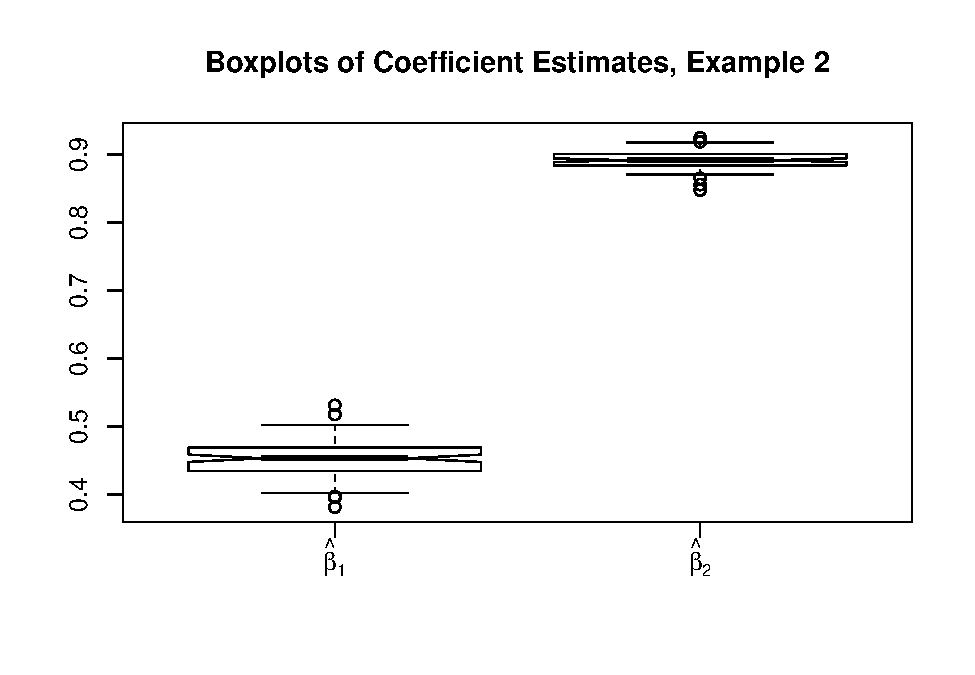
\includegraphics[width=10cm]{siqr_files/figure-latex/unnamed-chunk-14-1} 

\end{Schunk}

Similarly, we plot the estimated quantiles and their 95\% point-wise confidence bounds with the provided plot function $plot.siqr$. The observed data points are also plotted. 

\begin{Schunk}
\begin{Sinput}
  est.sim.50 <- siqr(data$Y[[1]],data$X,beta.inital = NULL, tau=0.5)
  plot.siqr(est.sim.50,bootstrap.interval = TRUE)
\end{Sinput}

\centering
\addtolength{\leftskip} {-2cm}
\addtolength{\rightskip}{-2cm}
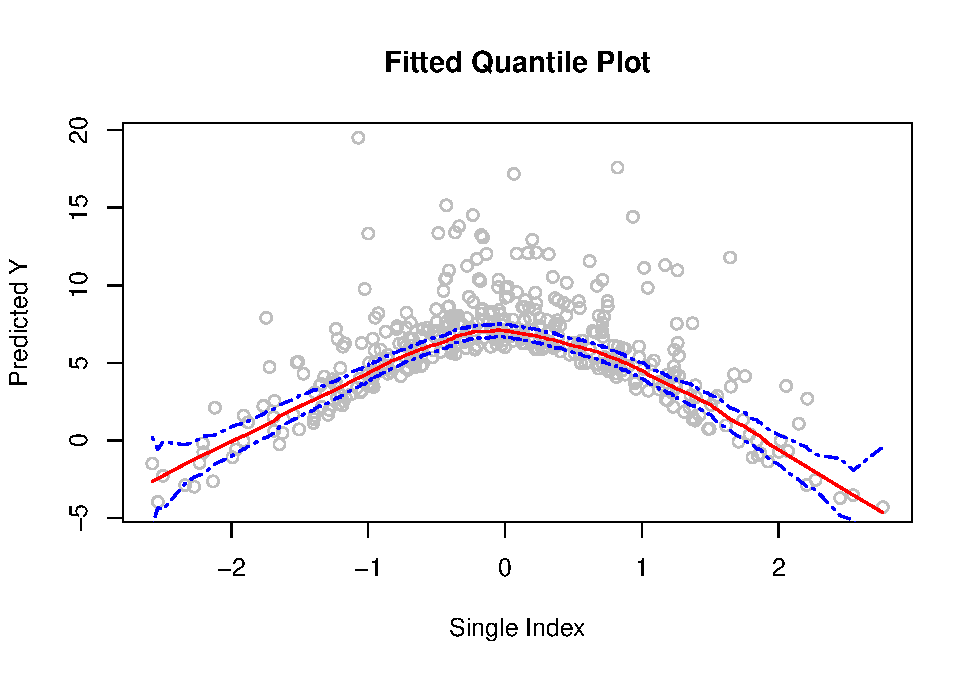
\includegraphics[width=10cm]{siqr_files/figure-latex/unnamed-chunk-15-1}

\end{Schunk}

\section{Summary}
In this paper, we present the R package \pkg{SIQR} for the local linear approach to single-index quantile regression models in \cite{wu_single-index_2010}. We demonstrate the package applications to a popular Boston-housing data application and two simulation studies. It is our hope that the package will be useful to a variety of applications, especially for complex heterogeneous data where flexible quantile regression modeling is desirable.
\bibliography{SIQR} 


\address{Tianhai Zu\\
  University of Cincinnati\\
  2906 Woodside Drive\\
  Cincinnati, OH 45221 \\
  (ORCiD if desired)\\
  \email{zuti@mail.uc.edu}}

\address{Yan Yu\\
	University of Cincinnati\\
	2906 Woodside Drive\\
	Cincinnati, OH 45221 \\
	https://orcid.org/0000-0002-2859-3093\\
	\email{Yan.YU@uc.edu}}





